\documentclass[border=2pt]{standalone}
% Figure style adopted from the reference figures of
%   Kapteyn, Pretorius & Willcox (2021), Nature Computational Science 1, 337-347 (Figs. 1, 3, 6), and
%   Torzoni et al. (2024), Computer Methods in Applied Mechanics and Engineering 418, 116584 (Fig. 1).
% Colours were sampled from the vector PDF of the reference; text uses the body font of the article (Times).
\usepackage[T1]{fontenc}
\usepackage{newtxtext,newtxmath}         % Times text and math; \sffamily = TeX Gyre Heros (Torzoni-style labels)
\usepackage{tikz}
\usetikzlibrary{positioning,arrows.meta,calc,fit,backgrounds,shapes.geometric,shapes.misc}
\usepackage{pgfplots}
\pgfplotsset{compat=1.18}
\usepgfplotslibrary{groupplots,fillbetween}
% ---- reference palette
\definecolor{ink}{HTML}{231F20}
\definecolor{inkS}{HTML}{464749}
\definecolor{inkM}{HTML}{808285}
\definecolor{inkL}{HTML}{A7A9AC}
\definecolor{gridc}{HTML}{BCBEC0}
\definecolor{physN}{HTML}{E6E7E8}   % physical state node
\definecolor{obsN}{HTML}{FED09E}    % observation node
\definecolor{ctlN}{HTML}{FBD9E8}    % control node
\definecolor{dtN}{HTML}{D0E6F7}     % digital state node
\definecolor{qoiN}{HTML}{FEEED5}    % quantity-of-interest node
\definecolor{rewN}{HTML}{D4EDEA}    % reward node
\definecolor{dtL}{HTML}{3953A4}     % digital-state estimate
\definecolor{dtB}{HTML}{D5E7F2}     % digital-state uncertainty band
\definecolor{obsL}{HTML}{F7941D}    % observational data
\definecolor{ctlL}{HTML}{EE287C}    % control inputs (lines)
\definecolor{ctlD}{HTML}{F49AC1}    % control inputs (dots)
\definecolor{rewL}{HTML}{066839}    % reward
\definecolor{cRed}{HTML}{BE1E2D}
\definecolor{seqLo}{HTML}{EEF4FA}
% ---- node styles of the dynamic decision network (Kapteyn et al., Fig. 3)
\tikzset{
  ddn/.style={draw=ink, line width=0.63pt, minimum size=0.52cm, inner sep=0pt, font=\small},
  nPhys/.style={ddn, circle, fill=physN},
  nObs/.style={ddn, circle, fill=obsN, line width=1.6pt},
  nCtl/.style={ddn, rectangle, fill=ctlN, line width=1.6pt, minimum size=0.47cm},
  nDig/.style={ddn, circle, fill=dtN},
  nQoi/.style={ddn, circle, fill=qoiN},
  nRew/.style={ddn, diamond, fill=rewN, minimum size=0.6cm},
  edge/.style={->, >={Stealth[length=3.2pt,width=2.6pt]}, draw=ink, line width=0.55pt},
}
% ---- plot style (Kapteyn et al., Fig. 6): quantity in the panel title, light horizontal grid, left/bottom axes only
\pgfplotsset{
  kstyle/.style={
    font=\footnotesize, scale only axis,
    axis x line*=bottom, axis y line*=left,
    axis line style={ink, line width=0.6pt}, tick style={ink, line width=0.5pt},
    tick align=outside, major tick length=2.2pt,
    ymajorgrids, major grid style={gridc, line width=0.3pt},
    tick label style={font=\footnotesize, text=ink}, label style={font=\footnotesize, text=ink},
    title style={font=\footnotesize, text=ink, at={(0,1)}, anchor=south west, xshift=-1pt, yshift=1pt},
    every axis plot/.append style={line width=1.0pt}, clip=false,
  },
}
\newcommand{\plabel}[1]{\textit{#1)}\ }

% Layout after Torzoni et al. (2024, Fig. 1): information loop around a central graphical model;
% node styles after Kapteyn et al. (2021, Fig. 3).
\begin{document}
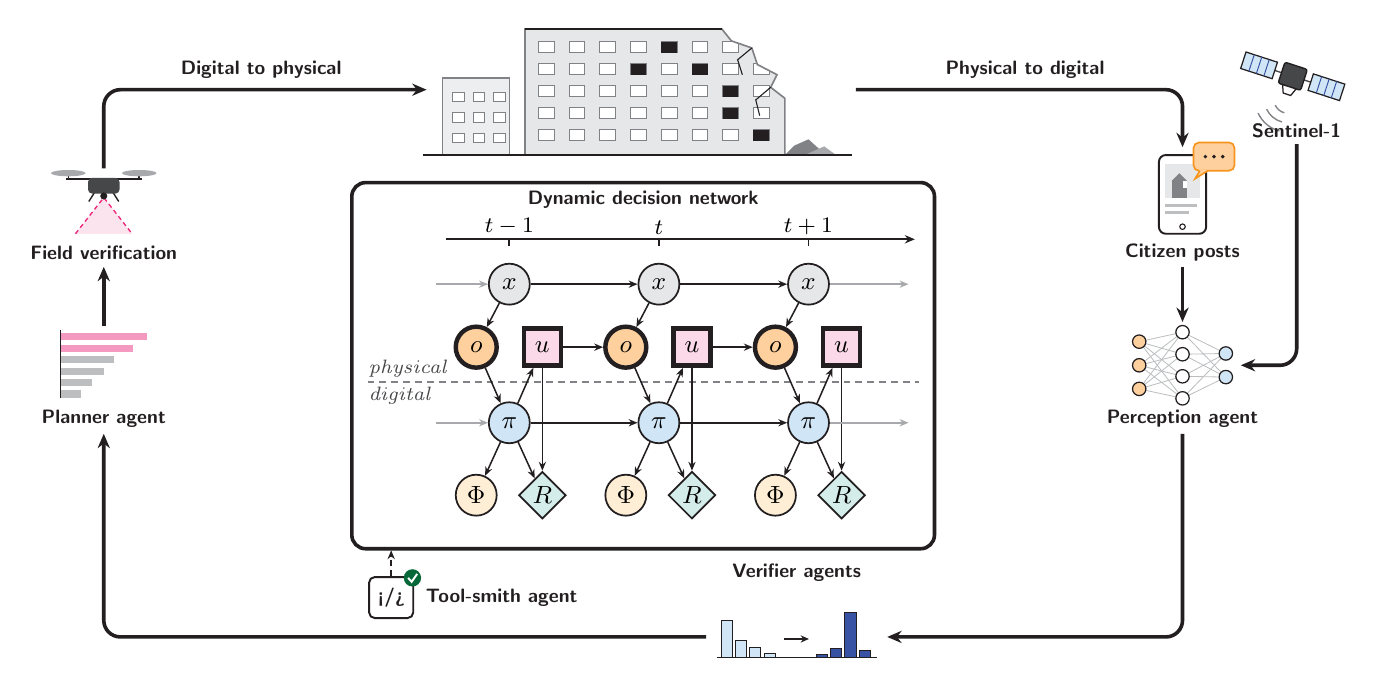
\begin{tikzpicture}[
  sec/.style={font=\sffamily\bfseries\scriptsize, text=ink, inner sep=1pt},
  ring/.style={->, >={Stealth[length=5.2pt,width=4.4pt]}, draw=ink, line width=1.3pt, rounded corners=6pt},
  thin/.style={draw=ink, line width=0.4pt},
]
% ============================================================ central dynamic decision network
\draw[ink, line width=1.3pt, rounded corners=5pt, fill=white] (4.55,1.62) rectangle (11.95,6.27);
\node[sec] at (8.25,6.05) {Dynamic decision network};
\draw[->, >={Stealth[length=3.6pt,width=3pt]}, ink, line width=0.6pt] (5.75,5.55) -- (11.7,5.55);
\foreach \x/\l in {6.55/{t-1}, 8.45/{t}, 10.35/{t+1}} {
  \draw[ink, line width=0.6pt] (\x,5.55) -- (\x,5.47);
  \node[font=\footnotesize, inner sep=1pt, anchor=south] at (\x,5.57) {$\l$};
}
\draw[inkM, line width=0.5pt, dash pattern=on 2.5pt off 1.8pt] (4.75,3.74) -- (11.75,3.74);
\node[font=\scriptsize\itshape, text=inkS, anchor=south west, inner sep=1pt] at (4.72,3.76) {physical};
\node[font=\scriptsize\itshape, text=inkS, anchor=north west, inner sep=1pt] at (4.72,3.72) {digital};
\foreach \i/\x/\t in {0/6.55/{t-1}, 1/8.45/{t}, 2/10.35/{t+1}} {
  \node[nPhys] (x\i) at (\x,4.98) {$x$};
  \node[nObs]  (o\i) at ($(\x,4.18)+(-0.42,0)$) {$o$};
  \node[nCtl]  (u\i) at ($(\x,4.18)+(0.42,0)$) {$u$};
  \node[nDig]  (p\i) at (\x,3.22) {$\pi$};
  \node[nQoi]  (f\i) at ($(\x,2.3)+(-0.42,0)$) {$\Phi$};
  \node[nRew]  (r\i) at ($(\x,2.3)+(0.42,0)$) {$R$};
  \draw[edge] (x\i) -- (o\i);
  \draw[edge] (o\i) -- (p\i);
  \draw[edge] (p\i) -- (u\i);
  \draw[edge] (p\i) -- (f\i);
  \draw[edge] (p\i) -- (r\i);
  \draw[edge] (u\i) -- (r\i);
}
\foreach \a/\b in {0/1, 1/2} {
  \draw[edge] (x\a) -- (x\b);
  \draw[edge] (p\a) -- (p\b);
  \draw[edge] (u\a) -- (o\b);
}
\draw[edge, draw=inkL] (5.62,4.98) -- (x0);
\draw[edge, draw=inkL] (x2) -- (11.62,4.98);
\draw[edge, draw=inkL] (5.62,3.22) -- (p0);
\draw[edge, draw=inkL] (p2) -- (11.62,3.22);
% ============================================================ physical asset (top)
\begin{scope}[shift={(6.75,6.62)}]
  % neighbouring intact building
  \fill[physN!70] (-1.05,0) rectangle (-0.2,0.98);
  \draw[inkM, line width=0.5pt] (-1.05,0) rectangle (-0.2,0.98);
  \foreach \c in {0,1,2} \foreach \r in {0,1,2}
    \draw[inkM, line width=0.3pt, fill=white] (-0.92+\c*0.26,0.16+\r*0.26) rectangle ++(0.15,0.12);
  % damaged block
  \path[fill=physN] (0,0) -- (3.3,0) -- (3.3,0.72) -- (3.12,0.86) -- (3.2,1.02) -- (2.95,1.15) -- (2.88,1.36)
        -- (2.62,1.45) -- (2.5,1.6) -- (0,1.6) -- cycle;
  \begin{scope}
    \clip (0,0) -- (3.3,0) -- (3.3,0.72) -- (3.12,0.86) -- (3.2,1.02) -- (2.95,1.15) -- (2.88,1.36)
          -- (2.62,1.45) -- (2.5,1.6) -- (0,1.6) -- cycle;
    \foreach \c in {0,...,7} \foreach \r in {0,...,4}
      \draw[inkM, line width=0.3pt, fill=white] (0.17+\c*0.39,0.18+\r*0.28) rectangle ++(0.2,0.14);
    \foreach \c/\r in {5/3, 6/1, 4/4, 6/2, 7/0, 3/3}
      \fill[ink] (0.17+\c*0.39,0.18+\r*0.28) rectangle ++(0.2,0.14);
  \end{scope}
  \draw[inkM, line width=0.6pt] (0,0) -- (3.3,0) -- (3.3,0.72) -- (3.12,0.86) -- (3.2,1.02) -- (2.95,1.15) -- (2.88,1.36)
        -- (2.62,1.45) -- (2.5,1.6) -- (0,1.6) -- cycle;
  \draw[ink, line width=1.0pt] (0,1.6) -- (2.5,1.6);
  \draw[ink, line width=0.4pt] (3.12,0.86) -- (2.93,0.7) -- (2.98,0.5);
  \draw[ink, line width=0.4pt] (2.88,1.36) -- (2.7,1.21) -- (2.76,1.02);
  \fill[inkM] (3.3,0) -- (3.82,0) -- (3.6,0.2) -- (3.42,0.12) -- cycle;
  \fill[inkL] (3.55,0) -- (3.95,0) -- (3.8,0.11) -- cycle;
  \draw[ink, line width=0.6pt] (-1.3,0) -- (4.15,0);
\end{scope}
% ============================================================ right column: physical -> digital
% citizen posts (phone + post bubble)
\begin{scope}[shift={(15.1,6.12)}]
  \draw[ink, line width=0.7pt, rounded corners=2.5pt, fill=white] (-0.3,-0.5) rectangle (0.3,0.5);
  \fill[physN] (-0.22,-0.04) rectangle (0.22,0.38);
  \fill[inkM] (-0.14,-0.04) rectangle (0.06,0.17); \fill[inkM] (-0.14,0.17) -- (-0.04,0.27) -- (0.06,0.17) -- cycle;
  \fill[white] (0.0,0.08) rectangle (0.06,0.17);
  \fill[gridc] (-0.22,-0.16) rectangle (0.18,-0.12);
  \fill[gridc] (-0.22,-0.25) rectangle (0.08,-0.21);
  \draw[ink, line width=0.4pt] (0,-0.41) circle (0.035);
  \draw[obsL, line width=0.6pt, fill=obsN, rounded corners=2pt] (0.14,0.3) -- (0.66,0.3) -- (0.66,0.66) -- (0.14,0.66) -- cycle;
  \fill[obsN] (0.22,0.31) -- (0.16,0.2) -- (0.32,0.31) -- cycle;
  \draw[obsL, line width=0.6pt] (0.22,0.3) -- (0.16,0.2) -- (0.32,0.3);
  \foreach \d in {0.29,0.4,0.51} \fill[ink] (\d,0.48) circle (0.025);
\end{scope}
\node[sec] at (15.1,5.38) {Citizen posts};
% perception agent (network icon)
\begin{scope}[shift={(15.1,3.95)}]
  \foreach \a in {-0.3,0,0.3} \foreach \b in {-0.42,-0.14,0.14,0.42} \draw[gridc, line width=0.3pt] (-0.55,\a) -- (0,\b);
  \foreach \b in {-0.42,-0.14,0.14,0.42} \foreach \c in {-0.15,0.15} \draw[gridc, line width=0.3pt] (0,\b) -- (0.55,\c);
  \foreach \a in {-0.3,0,0.3} \draw[ink, line width=0.45pt, fill=obsN] (-0.55,\a) circle (0.085);
  \foreach \b in {-0.42,-0.14,0.14,0.42} \draw[ink, line width=0.45pt, fill=white] (0,\b) circle (0.085);
  \foreach \c in {-0.15,0.15} \draw[ink, line width=0.45pt, fill=dtN] (0.55,\c) circle (0.085);
\end{scope}
\node[sec] at (15.1,3.27) {Perception agent};
% satellite radar (Sentinel-1): second, systematic observation source
\begin{scope}[shift={(16.5,7.62)}, rotate=-18]
  \foreach \s in {-1,1} {
    \draw[inkS, line width=0.5pt] (\s*0.15,0) -- (\s*0.24,0);
    \draw[ink, line width=0.45pt, fill=dtN] (\s*0.24,-0.11) rectangle (\s*0.66,0.11);
    \foreach \g in {0.35,0.45,0.55} \draw[dtL, line width=0.35pt] (\s*\g,-0.11) -- (\s*\g,0.11);
  }
  \draw[ink, line width=0.5pt, fill=inkS, rounded corners=0.8pt] (-0.15,-0.14) rectangle (0.15,0.14);
  \draw[ink, line width=0.45pt, fill=white] (-0.09,-0.14) -- (0.09,-0.14) -- (0.05,-0.24) -- (-0.05,-0.24) -- cycle;
\end{scope}
\foreach \r in {0.18,0.3,0.42} \draw[inkM, line width=0.5pt] ($(16.44,7.33)+(205:\r)$) arc[start angle=205, end angle=255, radius=\r];
\node[sec] at (16.55,6.93) {Sentinel-1};
% ============================================================ left column: digital -> physical
% field verification (UAV with inspection beam)
\begin{scope}[shift={(1.4,6.2)}]
  \fill[ctlN, opacity=0.7] (0,-0.12) -- (-0.36,-0.58) -- (0.36,-0.58) -- cycle;
  \draw[ctlL, line width=0.5pt, dash pattern=on 1.6pt off 1.2pt] (-0.36,-0.58) -- (0,-0.12) -- (0.36,-0.58);
  \draw[ink, line width=0.7pt] (-0.48,0.12) -- (0.48,0.12);
  \foreach \s in {-1,1} {
    \draw[ink, line width=0.6pt] (\s*0.45,0.12) -- (\s*0.45,0.18);
    \fill[inkL] (\s*0.45,0.19) ellipse (0.22 and 0.04);
    \draw[ink, line width=0.5pt] (\s*0.12,-0.06) -- (\s*0.19,-0.17);
  }
  \fill[inkS, rounded corners=1.5pt] (-0.2,-0.07) rectangle (0.2,0.13);
  \fill[ink] (0,-0.1) circle (0.045);
\end{scope}
\node[sec] at (1.4,5.38) {Field verification};
% planner agent (ranked inspection priorities)
\begin{scope}[shift={(1.4,3.95)}]
  \foreach \i/\L in {0/1.0, 1/0.84, 2/0.62, 3/0.5, 4/0.36, 5/0.24} {
    \pgfmathsetmacro{\yy}{0.36-\i*0.145}
    \ifnum\i<2 \fill[ctlD] (-0.55,\yy-0.045) rectangle ++(\L*1.1,0.09);
    \else \fill[gridc] (-0.55,\yy-0.045) rectangle ++(\L*1.1,0.09); \fi
  }
  \draw[ink, line width=0.5pt] (-0.55,-0.42) -- (-0.55,0.45);
\end{scope}
\node[sec] at (1.4,3.27) {Planner agent};
% ============================================================ bottom: verifier agents and tool-smith agent
\begin{scope}[shift={(10.2,0.5)}, scale=1.3]
  \foreach \i/\h in {0/0.36, 1/0.17, 2/0.1, 3/0.04}
    \draw[ink, line width=0.3pt, fill=dtN] (-0.74+\i*0.14,-0.2) rectangle ++(0.11,\h);
  \draw[->, >={Stealth[length=3pt,width=2.6pt]}, ink, line width=0.6pt] (-0.12,-0.02) -- (0.12,-0.02);
  \foreach \i/\h in {0/0.03, 1/0.09, 2/0.44, 3/0.07}
    \draw[ink, line width=0.3pt, fill=dtL] (0.19+\i*0.14,-0.2) rectangle ++(0.11,\h);
  \draw[ink, line width=0.5pt] (-0.78,-0.2) -- (0.78,-0.2);
\end{scope}
\node[sec] at (10.2,1.32) {Verifier agents};
\begin{scope}[shift={(5.05,1.0)}]
  \draw[ink, line width=0.7pt, rounded corners=2pt, fill=white] (-0.28,-0.26) rectangle (0.28,0.26);
  \node[font=\sffamily\bfseries\scriptsize, text=ink] at (0,0) {</>};
  \fill[rewL] (0.27,0.25) circle (0.11);
  \draw[white, line width=0.7pt] (0.215,0.25) -- (0.26,0.2) -- (0.33,0.3);
\end{scope}
\node[sec, anchor=west] at (5.45,1.0) {Tool-smith agent};
\draw[->, >={Stealth[length=3.2pt,width=2.6pt]}, ink, line width=0.6pt, dash pattern=on 2pt off 1.5pt] (5.05,1.28) -- (5.05,1.6);
% ============================================================ information loop (clockwise)
\draw[ring] (10.95,7.45) -- (15.1,7.45) -- (15.1,6.72);
\draw[ring] (15.1,5.2) -- (15.1,4.5);
\draw[ring] (16.55,6.76) -- (16.55,3.95) -- (15.84,3.95);
\draw[ring] (15.1,3.08) -- (15.1,0.5) -- (11.35,0.5);
\draw[ring] (9.05,0.5) -- (1.4,0.5) -- (1.4,3.08);
\draw[ring] (1.4,4.45) -- (1.4,5.2);
\draw[ring] (1.4,6.45) -- (1.4,7.45) -- (5.5,7.45);
\node[sec, anchor=south] at (13.1,7.55) {Physical to digital};
\node[sec, anchor=south] at (3.4,7.55) {Digital to physical};
\end{tikzpicture}
\end{document}
